\documentclass{standalone}
\usepackage{tikz}
\usetikzlibrary{patterns, positioning}


\begin{document}
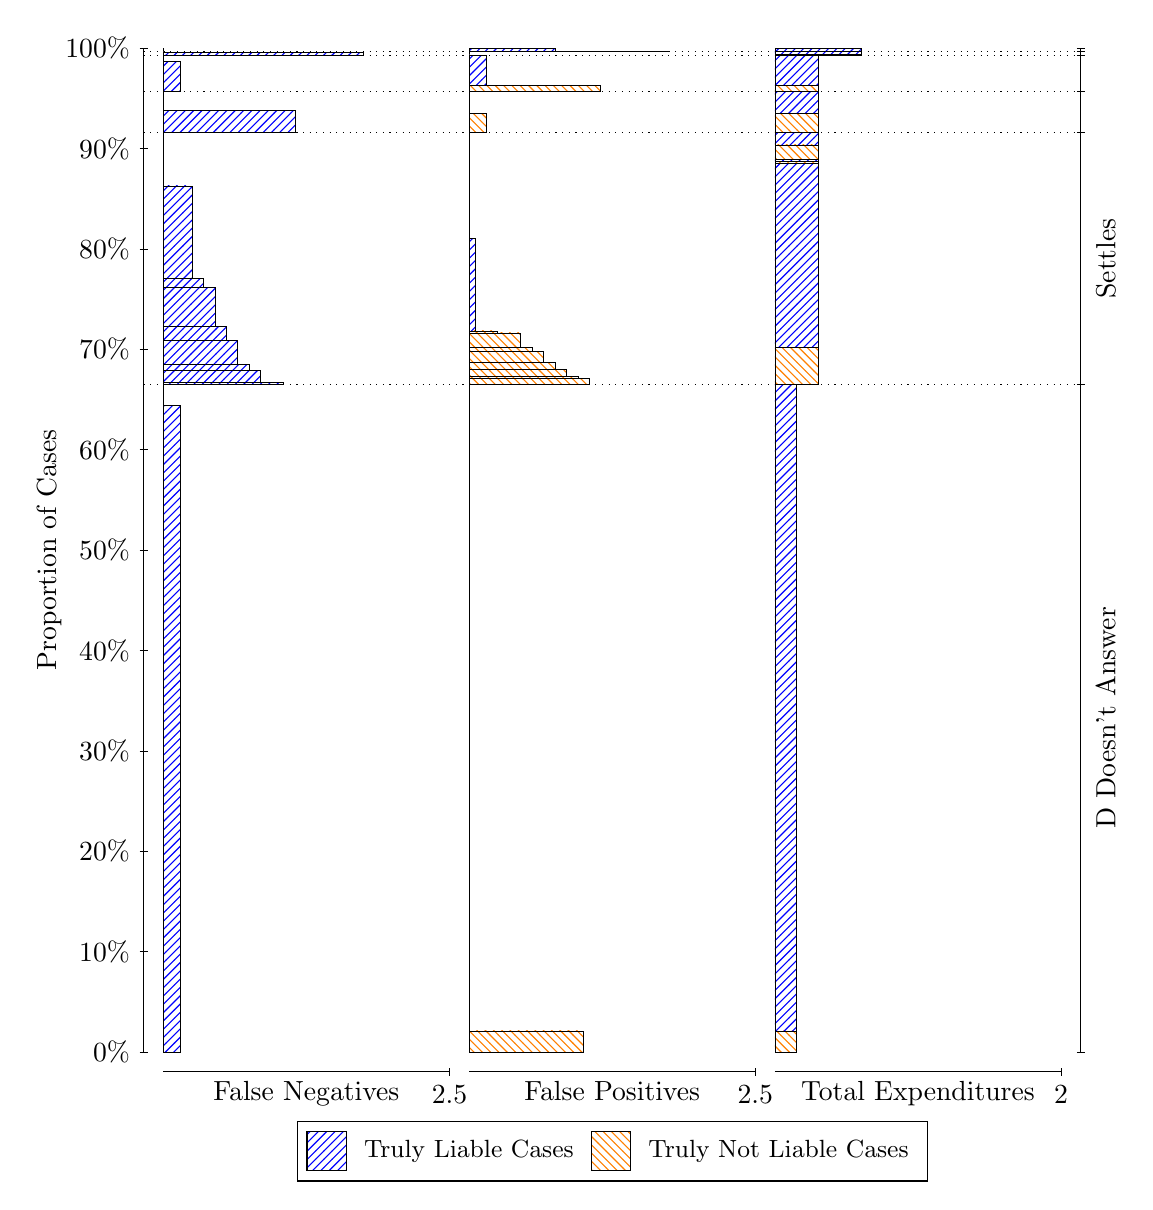
\begin{tikzpicture}
\draw[black, very thin] (1.5,1.75) -- (1.5,14.5);
\node[rotate=90, text=black, anchor=center] at (0.3, 8.125) {Proportion of Cases};
\draw[black, very thin] (1.45,1.75) -- (1.55,1.75);
\node[text=black, anchor=east] at (1.45, 1.75) {0\%};
\draw[black, very thin] (1.45,3.025) -- (1.55,3.025);
\node[text=black, anchor=east] at (1.45, 3.025) {10\%};
\draw[black, very thin] (1.45,4.3) -- (1.55,4.3);
\node[text=black, anchor=east] at (1.45, 4.3) {20\%};
\draw[black, very thin] (1.45,5.575) -- (1.55,5.575);
\node[text=black, anchor=east] at (1.45, 5.575) {30\%};
\draw[black, very thin] (1.45,6.85) -- (1.55,6.85);
\node[text=black, anchor=east] at (1.45, 6.85) {40\%};
\draw[black, very thin] (1.45,8.125) -- (1.55,8.125);
\node[text=black, anchor=east] at (1.45, 8.125) {50\%};
\draw[black, very thin] (1.45,9.4) -- (1.55,9.4);
\node[text=black, anchor=east] at (1.45, 9.4) {60\%};
\draw[black, very thin] (1.45,10.675) -- (1.55,10.675);
\node[text=black, anchor=east] at (1.45, 10.675) {70\%};
\draw[black, very thin] (1.45,11.95) -- (1.55,11.95);
\node[text=black, anchor=east] at (1.45, 11.95) {80\%};
\draw[black, very thin] (1.45,13.225) -- (1.55,13.225);
\node[text=black, anchor=east] at (1.45, 13.225) {90\%};
\draw[black, very thin] (1.45,14.5) -- (1.55,14.5);
\node[text=black, anchor=east] at (1.45, 14.5) {100\%};

\draw[black, very thin] (13.4,1.75) -- (13.4,14.5);
\draw[black, very thin] (13.35,1.75) -- (13.45,1.75);
\node[anchor=west] at (13.35, 1.75) {};
\draw[black, very thin] (13.35,10.232) -- (13.45,10.232);
\node[anchor=west] at (13.35, 10.232) {};
\draw[black, very thin] (13.35,13.425) -- (13.45,13.425);
\node[anchor=west] at (13.35, 13.425) {};
\draw[black, very thin] (13.35,13.95) -- (13.45,13.95);
\node[anchor=west] at (13.35, 13.95) {};
\draw[black, very thin] (13.35,14.406) -- (13.45,14.406);
\node[anchor=west] at (13.35, 14.406) {};
\draw[black, very thin] (13.35,14.456) -- (13.45,14.456);
\node[anchor=west] at (13.35, 14.456) {};
\draw[black, very thin] (13.35,14.5) -- (13.45,14.5);
\node[anchor=west] at (13.35, 14.5) {};

\draw[black, very thin, pattern color=blue, pattern=north east lines] (1.75,1.75) rectangle (1.968,9.965);
\draw[black, very thin, pattern color=orange, pattern=north west lines] (1.75,9.965) rectangle (1.75,10.232);
\draw[black, very thin, pattern color=blue, pattern=north east lines] (1.75,10.232) rectangle (3.276,10.251);
\draw[black, very thin, pattern color=blue, pattern=north east lines] (1.75,10.251) rectangle (2.9853,10.405);
\draw[black, very thin, pattern color=blue, pattern=north east lines] (1.75,10.405) rectangle (2.84,10.478);
\draw[black, very thin, pattern color=blue, pattern=north east lines] (1.75,10.478) rectangle (2.6947,10.784);
\draw[black, very thin, pattern color=blue, pattern=north east lines] (1.75,10.784) rectangle (2.5493,10.964);
\draw[black, very thin, pattern color=blue, pattern=north east lines] (1.75,10.964) rectangle (2.404,11.465);
\draw[black, very thin, pattern color=blue, pattern=north east lines] (1.75,11.465) rectangle (2.2587,11.57);
\draw[black, very thin, pattern color=blue, pattern=north east lines] (1.75,11.57) rectangle (2.1133,12.75);
\draw[black, very thin, pattern color=orange, pattern=north west lines] (1.75,12.75) rectangle (1.75,13.425);
\draw[black, very thin, pattern color=blue, pattern=north east lines] (1.75,13.425) rectangle (3.4213,13.709);
\draw[black, very thin, pattern color=orange, pattern=north west lines] (1.75,13.709) rectangle (1.75,13.95);
\draw[black, very thin, pattern color=blue, pattern=north east lines] (1.75,13.95) rectangle (1.968,14.332);
\draw[black, very thin, pattern color=orange, pattern=north west lines] (1.75,14.332) rectangle (1.75,14.406);
\draw[black, very thin, pattern color=blue, pattern=north east lines] (1.75,14.406) rectangle (4.2933,14.443);
\draw[black, very thin, pattern color=orange, pattern=north west lines] (1.75,14.443) rectangle (1.75,14.456);
\draw[black, very thin, pattern color=orange, pattern=north west lines] (1.75,14.456) rectangle (1.75,14.46);
\draw[black, very thin, pattern color=blue, pattern=north east lines] (1.75,14.46) rectangle (1.75,14.5);
\draw[black, very thin, pattern color=orange, pattern=north west lines] (5.6333,1.75) rectangle (7.0867,2.017);
\draw[black, very thin, pattern color=blue, pattern=north east lines] (5.6333,2.017) rectangle (5.6333,10.232);
\draw[black, very thin, pattern color=orange, pattern=north west lines] (5.6333,10.232) rectangle (7.1593,10.306);
\draw[black, very thin, pattern color=orange, pattern=north west lines] (5.6333,10.306) rectangle (7.014,10.325);
\draw[black, very thin, pattern color=orange, pattern=north west lines] (5.6333,10.325) rectangle (6.8687,10.414);
\draw[black, very thin, pattern color=orange, pattern=north west lines] (5.6333,10.414) rectangle (6.7233,10.503);
\draw[black, very thin, pattern color=orange, pattern=north west lines] (5.6333,10.503) rectangle (6.578,10.645);
\draw[black, very thin, pattern color=orange, pattern=north west lines] (5.6333,10.645) rectangle (6.4327,10.695);
\draw[black, very thin, pattern color=orange, pattern=north west lines] (5.6333,10.695) rectangle (6.4327,10.697);
\draw[black, very thin, pattern color=orange, pattern=north west lines] (5.6333,10.697) rectangle (6.2873,10.882);
\draw[black, very thin, pattern color=orange, pattern=north west lines] (5.6333,10.882) rectangle (5.9967,10.907);
\draw[black, very thin, pattern color=blue, pattern=north east lines] (5.6333,10.907) rectangle (5.706,12.087);
\draw[black, very thin, pattern color=blue, pattern=north east lines] (5.6333,12.087) rectangle (5.6333,13.425);
\draw[black, very thin, pattern color=orange, pattern=north west lines] (5.6333,13.425) rectangle (5.8513,13.666);
\draw[black, very thin, pattern color=blue, pattern=north east lines] (5.6333,13.666) rectangle (5.6333,13.95);
\draw[black, very thin, pattern color=orange, pattern=north west lines] (5.6333,13.95) rectangle (7.3047,14.024);
\draw[black, very thin, pattern color=blue, pattern=north east lines] (5.6333,14.024) rectangle (5.8513,14.406);
\draw[black, very thin, pattern color=orange, pattern=north west lines] (5.6333,14.406) rectangle (5.6333,14.42);
\draw[black, very thin, pattern color=blue, pattern=north east lines] (5.6333,14.42) rectangle (5.6333,14.456);
\draw[black, very thin, pattern color=orange, pattern=north west lines] (5.6333,14.456) rectangle (8.1767,14.46);
\draw[black, very thin, pattern color=blue, pattern=north east lines] (5.6333,14.46) rectangle (6.7233,14.5);
\draw[black, very thin, pattern color=orange, pattern=north west lines] (9.5167,1.75) rectangle (9.7892,2.017);
\draw[black, very thin, pattern color=blue, pattern=north east lines] (9.5167,2.017) rectangle (9.7892,10.232);
\draw[black, very thin, pattern color=orange, pattern=north west lines] (9.5167,10.232) rectangle (10.062,10.695);
\draw[black, very thin, pattern color=blue, pattern=north east lines] (9.5167,10.695) rectangle (10.062,13.039);
\draw[black, very thin, pattern color=orange, pattern=north west lines] (9.5167,13.039) rectangle (10.062,13.064);
\draw[black, very thin, pattern color=blue, pattern=north east lines] (9.5167,13.064) rectangle (10.062,13.083);
\draw[black, very thin, pattern color=orange, pattern=north west lines] (9.5167,13.083) rectangle (10.062,13.27);
\draw[black, very thin, pattern color=blue, pattern=north east lines] (9.5167,13.27) rectangle (10.062,13.425);
\draw[black, very thin, pattern color=orange, pattern=north west lines] (9.5167,13.425) rectangle (10.062,13.666);
\draw[black, very thin, pattern color=blue, pattern=north east lines] (9.5167,13.666) rectangle (10.062,13.95);
\draw[black, very thin, pattern color=orange, pattern=north west lines] (9.5167,13.95) rectangle (10.062,14.024);
\draw[black, very thin, pattern color=blue, pattern=north east lines] (9.5167,14.024) rectangle (10.062,14.406);
\draw[black, very thin, pattern color=orange, pattern=north west lines] (9.5167,14.406) rectangle (10.607,14.42);
\draw[black, very thin, pattern color=blue, pattern=north east lines] (9.5167,14.42) rectangle (10.607,14.456);
\draw[black, very thin, pattern color=orange, pattern=north west lines] (9.5167,14.456) rectangle (10.607,14.46);
\draw[black, very thin, pattern color=blue, pattern=north east lines] (9.5167,14.46) rectangle (10.607,14.5);
\draw[black, dotted] (1.5,10.232) -- (13.4,10.232);
\draw[black, dotted] (1.5,13.425) -- (13.4,13.425);
\draw[black, dotted] (1.5,13.95) -- (13.4,13.95);
\draw[black, dotted] (1.5,14.406) -- (13.4,14.406);
\draw[black, dotted] (1.5,14.456) -- (13.4,14.456);
\draw[black, very thin] (1.75,1.5) -- (5.3833,1.5);
\node[text=black, anchor=north] at (3.5667, 1.5) {False Negatives};
\draw[black, very thin] (5.3833,1.45) -- (5.3833,1.55);
\node[text=black, anchor=north] at (5.3833, 1.45) {2.5};

\draw[black, very thin] (5.6333,1.5) -- (9.2667,1.5);
\node[text=black, anchor=north] at (7.45, 1.5) {False Positives};
\draw[black, very thin] (9.2667,1.45) -- (9.2667,1.55);
\node[text=black, anchor=north] at (9.2667, 1.45) {2.5};

\draw[black, very thin] (9.5167,1.5) -- (13.15,1.5);
\node[text=black, anchor=north] at (11.333, 1.5) {Total Expenditures};
\draw[black, very thin] (13.15,1.45) -- (13.15,1.55);
\node[text=black, anchor=north] at (13.15, 1.45) {2};

\node[text=black, centered, rotate=90] at (13.72, 5.991) {D Doesn't Answer};
\node[text=black, centered, rotate=90] at (13.72, 11.828) {Settles};





\draw (7.449999999999999,1.5) node[draw=none] (baseCoordinate) {};
\begin{scope}[align=center]
        \matrix[scale=0.5, draw=black, below=0.5cm of baseCoordinate, nodes={draw}, column sep=0.1cm]{
            \node[rectangle, draw, minimum width=0.5cm, minimum height=0.5cm, pattern color=blue, pattern=north east lines] {}; &
            \node[draw=none, font=\small, text=black] (B) {Truly Liable Cases}; &
            \node[rectangle, draw, minimum width=0.5cm, minimum height=0.5cm, pattern color=orange, pattern=north west lines] {}; &
            \node[draw=none, font=\small, text=black] (B) {Truly Not Liable Cases}; \\
            };
\end{scope}

\end{tikzpicture}
\end{document}